\documentclass{IEEEtran}
\usepackage[ruled,vlined]{algorithm2e}
\usepackage{color,graphicx,epstopdf,changepage,amsmath,multirow}

\SetAlgoCaptionSeparator{.\space}
\renewcommand\AlCapFnt{\normalfont\scshape}
\setlength{\algomargin}{0.7cm}

\title{Comprehensive Quality-Aware Automated Semantic Web Service Composition}
 \author{Chen Wang, Hui Ma, Aaron Chen\\ School of
 Engineering and Computer Science, Victoria University of Wellington, New Zealand\\
Email: chen.wang@ecs.vuw.ac.nz, hui.ma@ecs.vuw.ac.nz, aaron.chen@ecs.vuw.ac.nz}

\usepackage[pdfauthor={\@author}, pdftitle={\@title}]{hyperref}
\makeatother

%\providecommand{\e}[1]{\ensuremath{\times 10^{#1}}}
\vspace{-1.5cm}

\begin{document}
\maketitle
\begin{abstract}
Semantic web service composition has been a prevailing research area in recent years. There are two major governance challenges faced by researchers (semantic matching and QoS optimisation). Semantic matchmaking aims to discover interoperable web services that can interact with each other to provide rich functionalities through language understanding and reasoning. QoS optimisation aims to meet non-functional requirement of service users. e.g minimum cost, maximal reliability. Many scholars have looked into nonfunctional optimisation problems in QoS-aware web service composition applying AI planning and Evolutionary Computation techniques. To meet users' requirement, one often needs to consider both semantic matching and QoS optimisation simultaneously. Existing works on web service composition often concerns either semantic service composition or QoS-aware service composition. However, there are very few works concerns both quality of semantic matchmaking and quality of services at the same time. Therefore, In this paper we consider two quality dimensions in a proposed more applicable comprehensive quality model for semantic web service composition, and present a automated semantic web service composition approach that can generate service composition solutions that meet both functional and non-functional requirement. We will evaluate our approach utilising a semantic benchmark dataset.

\end{abstract}
\vspace{-0.8cm}
\section{Introduction}\label{introduction}

\textit{Web service composition} pertains to a combination of multiple web services to provide a value-added composite service that accommodates customers' arbitrarily complex requirements. This application is developed by integrating interoperable and collaborative functionalities over heterogeneous systems. Due to the increase of the number of large-scale enterprise applications, the number of Web services has increased substantially and unprecedentedly. Therefore, manual and semi-automated web service composition are considered to be less efficient while automated web service composition enjoys less human intervention, less time consumption, and high productivity.

Two most notable challenges for web service composition are $(1)$ ensuring interoperability of services and $(2)$ achieving QoS optimisation \cite{fensel2011semantic}. \textit{Interoperability} of web services presents challenge $(1)$ in syntactic and semantics dimensions \cite{fensel2011semantic}. The syntactic dimension is covered by the XML-based technologies (such as $WSDL$, $SOAP$). The semantics aspect, on the other hand, demands further research. Through ontology-based semantics \cite{o2005review}, web services can understand and better collaborate with each other. There are many ontologies languages and formats for semantic service descriptions, such as OWL-S, WSML, and SAWSDL \cite{petrie2016web}, which make ``machine understanding'' possible through identifying and matching semantic similarity in input/output parameters of web services in heterogeneous environments. The second challenge $(2)$ is related to finding \textit{optimised solutions} to Quality of Service ($QoS$). This problem gives birth to \textit{QoS-aware service composition} that considers the composition of service-level agreements (SLA) \cite {sahai2002automated} involving a collection of SLA rules and policies for supporting QoS-based composition.

Existing works on service composition focus mainly on addressing the one of challenges above. A lot of works have been conducted to optimise the quality of compositions under a pre-defined abstract workflow, which is generally considered as \textit{semi-automated Web service composition} approach. Meanwhile, many research works consider the possibility of generating a composite plan automatically in discovering and selecting suitable web services, which are considered to be NP-hard \cite{moghaddam2014service}. \textit{Semantic web services composition} is distinguished from the syntactic service composition, with the hope of eliminating conflicts by the semantic level of web services. In the past few years, substantial works have been done on semantic web service composition \cite{fensel2011semantic,lecue2009optimizing}. However, few works have enabled truely automatic semantic web service composition, where both QoS and quality of semantic match making will be optimised simultaneously. To a given service request, the quality of service composition solution depends on both QoS and quality of semantic matchmaking. Therefore, a comprehensive quality model is needed to measure the quality of service composition solution.

The overall goal of this paper is to \textit{develop an comprehensive quality-aware automated semantic web service composition that satisfactorily optimises both functional and non-functional requirements}. Particularly, this paper extends existing works on semantic service composition and QoS-aware service composition by considering both QoS optimisation and semantic matching optimisation in our comprehensive quality model. Particle Swarm Optimisation (PSO) has show its promise in searching near-optimised service composition solution \cite{da2016particle}, we will propose a PSO-based service composition approach using our comprehensive quality model, which is considered to be more applicable way to measure semantic matchmaking in automated semantic web service composition. We will achieve three objectives in this work as follows:

\begin{enumerate}
 \item To propose a comprehensive quality model that address QoS and semantic matchmaking quality in considering different matching types with corresponding semantic similarity. This approach is consider to be a more applicable and effective way of finding an optimised solution in semantic web service composition.
  
 \item To propose a PSO-based service composition algorithm that utilises the proposed quality model. To do that we will first propose a representation of semantic service composition, which can model the quality of semantic matchmaking and QoS with the representation. A particle is then used to represent a queue of services that can be used to generate a near-optimised semantic service composition solution.
  
 \item To evaluate the performance of comprehensive quality awareness semantic web service composition by utilising benchmark datasets from Web Services Challenge 2009 (WSC09) \cite{kona2009wsc}. Also, we make a comparison between PSO-based and an existing GP-based approach employing our proposed comprehensive quality model.
 
\end{enumerate}

\section{Related Work} \label{relatedWork}
\textbf{Semantic web service matchmaking}. Substantial work \cite{bansal2016generalized,mier2015integrated,da2016particle,da2015graphevol,yu2013adaptive} on web service composition focused primarily on non-functional requirements consistently neglecting functional requirements. However few researchers addressed both functional and nonfunctional requirements at the same time in web service composition. To the best of our knowledge, \cite{fanjiang2014semantic,lecue2009optimizing,pop2009immune} reported some recent attempts on service composition that considers both nonfunctional (QoS) and functional (semantic) aspects. Semantic matchmaking utilises Description Logic($DL$) \cite{baader2003description} to search for services that ensure semantic matching utilising an ontology of the corresponding domain.

In \cite{shet2012new}, three approaches have been studied regarding the similarity measures using taxonomies: The first one is based on nodes, in which similarity is determined by the information content of the nodes; the second is entirely based on edge, where concept distance in a hierarchy structure is evaluated, and third one is the hybrid approach features a combination of these two. A similarity measure based on edge counting in taxonomy is introduced in \cite{shet2012new}. Neighbourhood concepts are considered in their model when $\lambda$ = 1 (default value as 0).

In \cite{lecue2009optimizing}, the quality of matchmaking problem is transferred to measure the quality of semantic links, one possible measure is applied to the degree of similarity using Common Description rate of a semantic link, where Extra Description and Least common subsume are required to be pre-calculated. Therefore, the quality of the semantic link is estimated as quality of matching types associated with their corresponding quality of Common Description rate. However, the weakness of semantic link quality is that calculation requires well and completely defined ontology in class, class axioms and properties. This makes it difficult to measure semantic matchmaking quality as it takes huge cost and time for the domain experts to establish required ontology. In comparison, we introduce a more applicable comprehensive quality model in a fully automated approach.

The work \cite{fanjiang2014semantic} concerns both functional and non-functional requirements in design time of semantic-based automatic service composition, where a GA-based approach with four unusual independent fitness functions are designed to solve the problems with these concerns. A sequence of fitness functions are used in the binary selection of chromosomes, rather than a single objective consisting of both functional and non-functional quality. Apart from that, match types are ignored in their quality evaluation of semantic matching.

\textbf{QoS-aware EC approaches}. Evolutionary Computation techniques are widely used to solve optimisation problems, where the search space is big, so that near-optimised solutions can be found in reasonable time. Genetic Programming (GP) \cite{da2016particle,da2015graphevol} is a typical EC technique applied to automated web service composition. GP-based approaches utilise tree representations, on which service and constructs are represented as terminal nodes and functional nodes respectively. The crossover and mutation operations reproduce various individuals while ensuring the correctness of structure. In \cite{yu2013adaptive}, the author optimises the overall quality of service composition by using a fitness function, which is also liable for the correctness in functionality through penalising infeasible solutions. Also, this paper increase the mutation rate while encountering low diversity in the population and adopt a higher crossover probability while trapped in local optimisation.

A hyper approach employs both a greedy search algorithm and genetic programming is introduced in \cite{ma2015hybrid} to generate locally optimised solution with functionality correctness. In particularly, the greedy search is used to the directed acrylic graph as composite solutions, which is further transferred to tree structure using unfolding techniques as the first generation in GP. In each individual,  terminal nodes are considered as task inputs,  root node as outputs, and inner nodes as atomic web services. During the reproduction process,  a randomly selected node in one individual is replaced with a new subtree generated by a greedy search to perform mutation while same atomic inner nodes in two random chosen individuals are swapped to perform crossover.

To simplify the checking of constraints for solutions, an indirect PSO-based approach was introduced in \cite{da2016particle}. A general graph is used as representation as composite solution in their PSO algorithm considering QoS optimisation. However, this solution does not consider distinguished matchmaking quality, which could lead to over-general outputs to be produced by selected services. In fact, customers' perspectives, application domains and ontology granularity all could have significant impact on the outputs requested by users. In some scenarios, the output is too broad to bear any specific meaning for the customers, even though those web services selected leads to a very good overall QoS. Therefore, we fill the gap by considering different matching types and parameter similarity to determine the overall quality of web service composition. Weighed graphs are also utilised in PSP to facilitate a new representation of web service composition adopted from \cite{da2016particle}.
\section{Problem Description}\label{problemDes}

The purpose of web service composition is to accomplish an arbitrarily complex task fulfilling customer's requirement, which could be denoted as a composite goal: $Comp.G(F(T_{Input}, T_{Output}), NF(T_{QoS}))$. This overall composite goal is demonstrated in two parts. The first functional part focus on transfering a given task input or input set to the desired Task output or output set. It typically refers to users' functional requirement. Another nonfunctional part specifies the acceptable level of composite quality of service. To accomplish the composite goal, two stages are involved: services discovery and service selection. Firstly, service discovery is to find matched web service: $S_{n}(F(S_{Input}, S_{Output}), NF(S_{QoS}))$ from a Service Repository: $S =  \{S_{1}, S_{2},..., S_{n} \}$ with the given $T_{Input}$. If no atomic web service could satisfy the composite goal, a combination of web services will be found to meet $Comp.G$. To ensure the composite solution returns the desired $Comp.G$, we consider a comprehensive quality model for service discovery and selection, where challenges $(1)$ and $(2)$ mentioned in Sect. \ref{introduction} are also addressed in Sect. \ref{qswsc_approach}.

\subsection{Semantic Web Service matchmaking Type}\label{semantic Web service Discovery}
The semantic service matchmaking aims to discover appropriate services from service repository in view of customers' functional requests. A semantic web service is defined by $S(F(S_{Input}\in C_{1}, S_{Output}\in C_{2}), NF(S_{QoS}))$, where both Input and Output are linked to concept $C_{1}$ and $C_{2}$ in an ontology ($O$) respectively, satisfying $O=\{C, Taxonomy\}$. A web service matching process is to match the output and input concepts of two services according to the Taxonomy within an Ontology (O). To measure the quality of semantic matchmaking, different matching levels are typically considered in the literature \cite{paolucci2002semantic}. To understand these levels, let us define two web services associated with concept-related parameters in a particular domain. $S_{1}$ $(F(S_{Input}\in C_{1}, S_{Outputs}\in C_{2}), NF(S_{QoS}))$ and  $S_{2}$ $(F(S_{Input}\in C_{3}, S_{Output}\in C_{4}), NF(S_{QoS}))$ and an Ontology($O$) with $C_{1},C_{2},C_{3}$, and $C_{4}$. The matching levels to be considered are:

\begin{itemize}
\item \textit{Exact} ($\equiv$): Output of Web service $S_{1}$ and Input of Web service $S_{2}$ are Exact match ($ S_{output} \in S_{1} \equiv S_{input}S_{2}$), if  Concept $C_{2}$ and Concept $C_{3}$ are equivalent.
\item \textit{Plugin} ($\sqsubseteq_{n}$): Output of Web service $S_{1}$ and Input of Web service $S_{2}$ are Plugin match ($S_{output} \in S_{1} \sqsubseteq_{n} S_{input} \in S_{2}$), if  Concept $C_{2}$ is a sub-concept of Concept $C_{3}$, and $n = \{1,2,...,n \}$ presents the levels of children concepts ($n=1$ stands for direct children).
\item \textit{Subsume} ($\sqsupseteq_{n}$): Output of Web service $S_{1}$ and Input of Web service $S_{2}$ are Subsume matched($S_{output} \in S_{1} \sqsupseteq_{n} S_{input} \in S_{2}$), if  Concept $C_{2}$ is a sub-concept of  Concept $C_{3}$, and $n = \{1,2,...,n \}$ presents the levels of parent concepts ($n=1$ stands for direct parent).
\item \textit{Fail} ($\perp$). Output of Web service $S_{1}$ and Input of Web service $S_{2}$ are not matched (Fail) ($S_{output} \in S_{1} \perp S_{input} \in S_{2}$), if none of the previous matches discovered.
\end{itemize}
\vspace{-0.5cm}
\subsection{Quality of Service and Composition Constructs}\label{Quality of Service and Composition Constructs}
Currently, most of the optimisation problems \cite{feng2013dynamic,huang2009effective,ma2015hybrid,da2014graph} in web service composition are focusing on QoS, which covers aspects in non-functional requirements. This problem has been explored in both single objective and multi-objectives optimisation problems. Customers prefer lowest execution cost with highest response time and reliability that could be optimised simultaneously. According to \cite{zeng2003quality}, four most often considered QoS parameters are as follows:
\begin{itemize}
\item \textit{Response time} ($T$) measures the expected delay in seconds between the moment when a request is sent and the moment when the results are received.
\item \textit{Cost} ($C$) is the amount of money that a service requester has to pay for executing the web service
\item \textit{Reliability} ($R$) is the probability that a request is correctly responded within the maximum expected time frame.
\item \textit{Availability} ($A$) is the probability that a web service is accessible.
\end{itemize}
The aggregation value of QoS attributes for web services composition varies with respect to different constructs, which reflects how services associated with each other in a service composition \cite{zeng2003quality}. Here we consider two composite constructs: sequence and parallel constructs, in building the composite web service. The QoS calculation models are described as follows:

\begin{figure}[h]
\centerline{
\fbox{
\begin{tabular}{p{0.6\linewidth}}
\space\hfill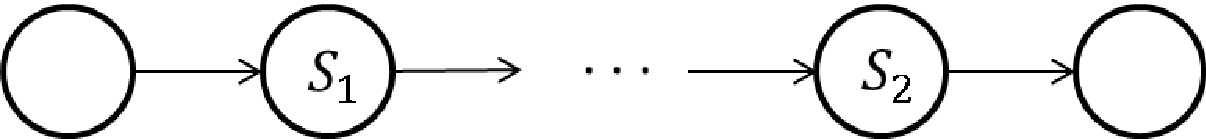
\includegraphics[width=2in]{sequence.pdf}\hfill\space\\[0.2cm]
$T=\sum\limits^m_{n=1}t_n$ \hfill $C=\sum\limits^m_{n=1}c_n$ \hfill
$A=\prod\limits^m_{n=1}a_n$ \hfill $R=\prod\limits^m_{n=1}r_n$
\end{tabular}}}
\caption{Sequence construct and calculation of its QoS properties
\cite{yu2013adaptive}.}
\label{sequence}
%\end{figure}
\vspace{0.3cm}
%\begin{figure}
\centerline{
\fbox{
\begin{tabular}{p{0.6\linewidth}}
\space\hfill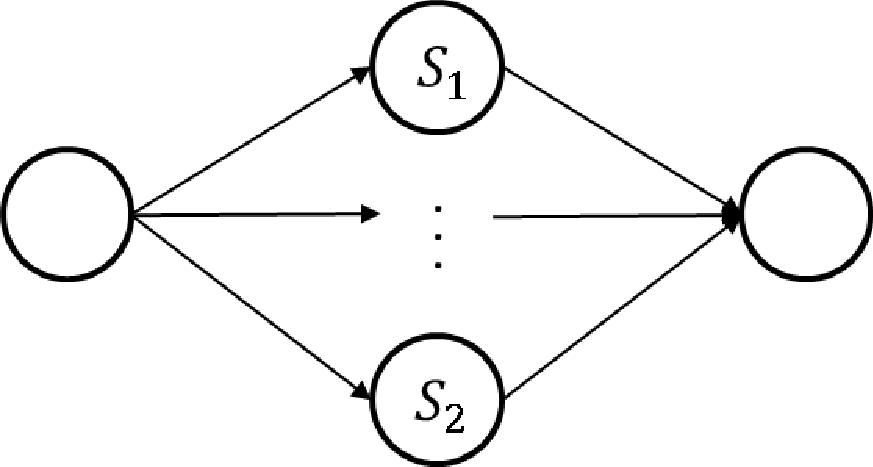
\includegraphics[width=1.4in]{parallel.pdf}\hfill\space\\[0.2cm]
\space\hfill$T=MAX\{t_n|n\in\{1,\ldots,m\}\}$\hfill\space\\[0.2cm]
$C=\sum\limits^m_{n=1}c_n$ \hfill $A=\prod\limits^m_{n=1}a_n$ \hfill
$R=\prod\limits^m_{n=1}r_n$
\end{tabular}}}
\caption{Parallel construct and calculation of its QoS properties
\cite{yu2013adaptive}.}
\label{parallel}
\end{figure}
\subsubsection{Sequence construct}
The composite web service executes each atomic service associated with a sequence construct in a definite sequence order. The aggregation value for total time ($T$) and total cost ($C$) is as the sum of time and cost of web services involved respectively. The overall availability and reliability in a sequence construct are calculated by multiplying their corresponding availability and reliability of each web service in probability theory. This construct is shown in Fig. \ref{sequence}.
\subsubsection{Parallel construct}
Web services in a parallel construct are executed concurrently. The QoS aggregation value for total cost, availability and reliability are the same as these in sequence construct while the Total time ($T$) is determined by the most time-consuming path in the composite flow of the solution. This construct is presented in Fig. \ref{parallel}.

\section{Comprehensive quality-aware Semantic Automated Web Service Composition}\label{qswsc_approach}

\begin{figure*}[h]
\centering
\fbox{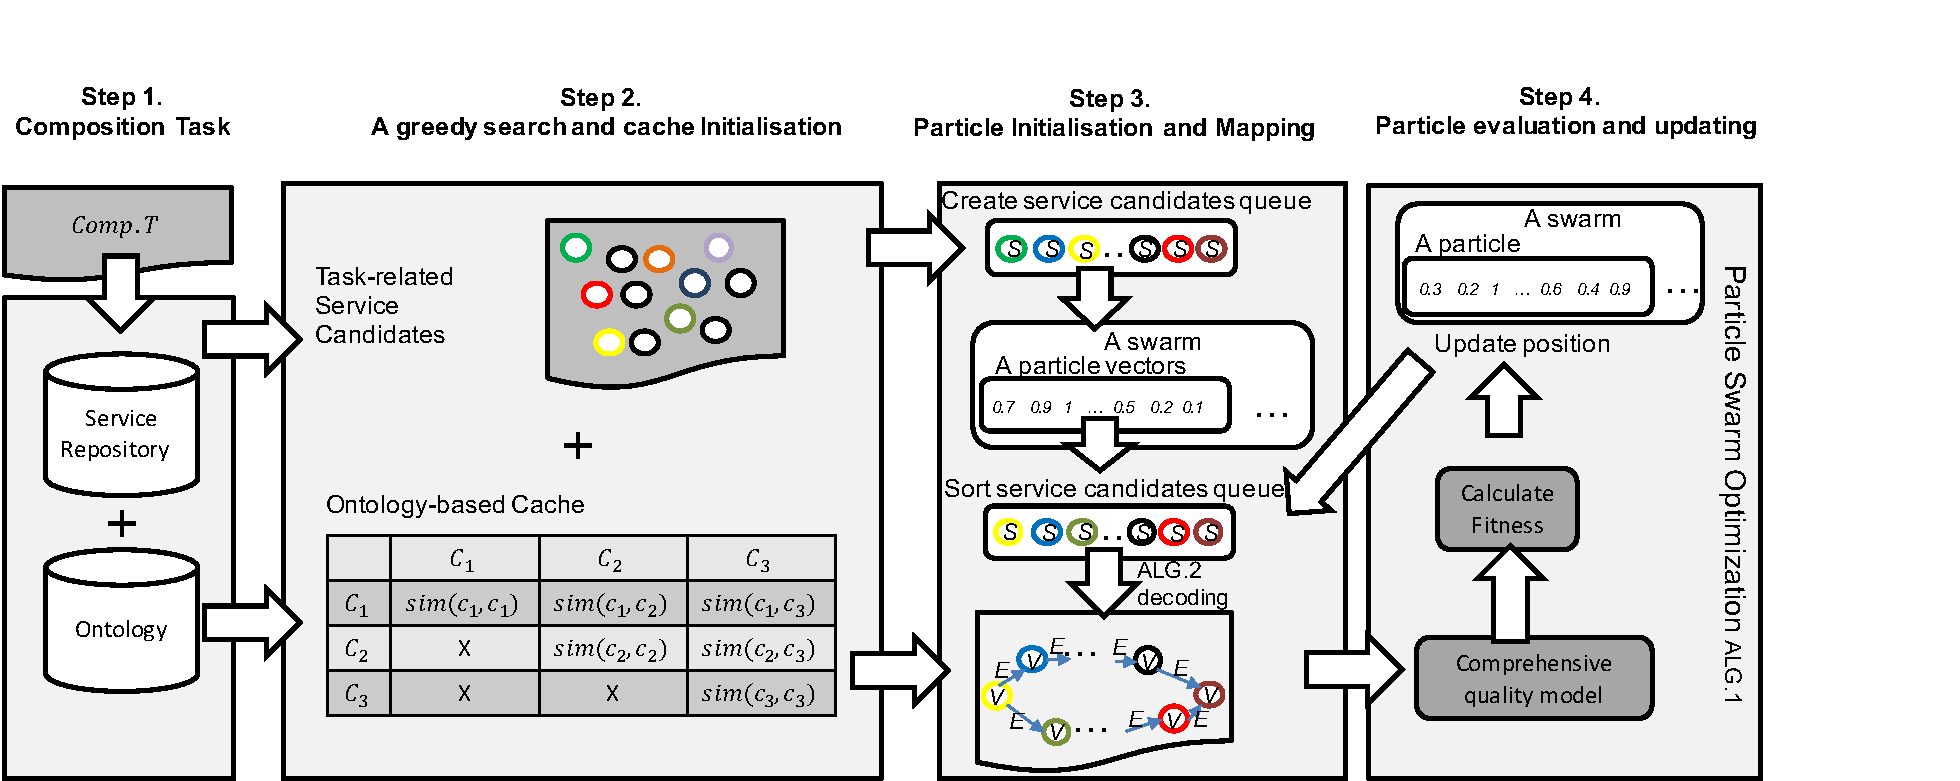
\includegraphics[scale=.4]{overview.pdf}}
 \caption{Overview of the proposed approach.}
 \label{overview}
\end{figure*}

In this section, we propose a comprehensive quality model for automated semantic service composition, and optimise both the quality of semantic matchmaking and QoS. PSO has shown its efficiency in solving combinatorial optimisation problems \cite{fukuyama2008fundamentals}. Therefore, we will employ a PSO-based approach, which is considered to be simple and efficient without penalising or repairing that often required by GP \cite{da2016particle}. Fig. \ref{overview} shows the overview of our approach with five steps. Step 1: The composite process is triggered by a composite goal defined in Subsection \ref{problemDes}, which describes customers requirements both functional and non-functional. Step 2: This composition goal are used to discover all relevant web services, which lead to a shrunken service repository that is subsequently used by PSO as a searching space. Step 3: A weighted graph representation is randomly built up from the an initial service queue that mapped to the particle's location, interleaving with semantic matchmaking process. In the weighted graph, graph edges are assigned with semantic matchmaking quality as weights. Step 4: The fitness value of the weighted graph is evaluated to update the position of particle under PSO algorithm in Sect. \ref{pso_algorithm}, where the position is mapped to the index of service queue. later on, the updated service queue is used to decode a new weighted graph as the composition solution. Step 4. Lastly, the best position found in the searching space is selected and decode into the final optimised solution. This PSO-based approach is different from \cite{da2016particle}, as we use weighted graphs as solution presentation.
\subsection{Semantic Matchmaking} \label{semantic_matchmaking}
To perform semantic matchmaking, we transfer a function match between $S_{1}: S_{output} \in C_{1}$ and $S_{2}:S_{output} \in S_{b}$ to a pair of concept match demonstrated in Sect. \ref{semantic Web service Discovery}. The matching process attempts to determine semantic matching between the source concepts of $C_{1}$ and the target concepts of $C_{2}$. Meanwhile, the quality of matched concepts are calculated in the quality model in subSection \ref{qualityModel}. The purpose of semantic matchmaking is to find more component services that could also potentially satisfy the quality of QoS with good functional quality.

The semantic matchmaking is achieved by utilising OWL2 and OWL-S or other semantic markup languages for web services. In this paper, we use MECE (Mediation Contract Extension) \cite{bleul2008self} and OWL-DL. MECE is considered to be an alternative semantic annotation for WSDL. MECE defines the service-related inputs and outputs with parameter-related concepts. OWL-DL is a sublanguage of OWL extended from RDF. It specifies semantic information of concepts involved in MECE. 

\subsection{Ontology-based Index Cached Optimisation}
In PSO, particles represent weighted graphs with edges and vertices associated with quality of semantic matchmaking and QoS respectively, the bottlenecks of generating weighted graph lie in building edges and nodes, which are related to the cost of semantic quality calculation and the size of service repository respectively. To effectively construct weighted graphs, we pre-calculate semantic matchmaking quality and mark the input-parameter concepts with a set of services. The key idea of the index is to create a mapping from the output-related concepts to matched input-related services while considering different levels of match types. Furthermore, this index size could also be reduced by only considering parameter-related concepts in the shrunken service repository, which contains  those task-relevant web services. This optimised cache also contributes to less and constant time for weighted graph building for the whole evolutionary process.

\subsection{Comprehensive Quality Model and Aggregation Matrix}\label{qualityModel}
In this paper, we propose a comprehensive quality model to evaluate the overall quality of semantic web service composition. This model overcome the disadvantages of current prevailing QoS-aware optimisation \cite{bansal2016generalized,mier2015integrated,da2016particle,da2015graphevol,yu2013adaptive} that ignores quality of semantic matchmaking.

\textbf{Semantic matchmaking model}. Due to the discretisational characteristics of different match types and values assigned to matching types that driven by the cost of data integration and manipulation \cite{lecue2009optimizing}, partial ordering match types are considered to be one factor for the semantic matchmaking quality. For example, Exact matching type demands less time for computation compared to that of Plugin match. Another factor in our proposed model is concept similarity, which could be evaluated based on the edge counting method defined in \cite{shet2012new}. This formula (\ref{equation1}) is used to estimate the similarity between parameter-related output concept and parameter-related input concept for selecting web services. Therefore, given the quality match type and the similarity of two parameters-related concepts, the semantic matchmaking quality of matched parameters is defined by Formula (\ref{equation2}), where the value of $q(p_ {mt})$ follows the same settings in \cite{lecue2009optimizing}. Particularly, 1 (Exact), 0.75 (Plugin), 0.5 (Subsume) or 0.25 (Intersection). 

\begin{equation}
q(p_ {s}){=} \frac{2N \cdot e^{-\lambda L/D} }{N_{1}+N_{2}}
\label{equation1}
\end{equation}

\begin{equation}
\label{equation2}
q(p_{sm}) \stackrel{.}{=} (q(p_ {mt}), \  q(p_ {s}))
\end{equation}

Further more, edges represent services connections in our weighted graph representations, where assigned weight value $q(e_{sm})$ is considered to be semantic matching quality on edge level according to parameter aggregations. The weight value $q(e_{sm})$ is defined in \ref{equation3}, where $q(e_ {mt})$ and $q(e_ {s})$ are the average value of concept-related parameters quality in $q(p_{mt})$ and $q(p_{s})$ respectively. 

\begin{equation}
\label{equation3}
q(e_{sm}) \stackrel{.}{=} (q(e_ {mt}), \  q(e_ {s}))
\end{equation}

\textbf{Comprehensive quality model}. Compared to QoS evaluation model, the comprehensive quality model is established to investigate both functional and non-functional requirements. The comprehensive quality of our service composition representation refers to QoS of service vertices and Semantic matching quality of Edges in weighted graphs. Consequently, the comprehensive quality model is defined in Formula (\ref{equation4}), which could be further broken down into Formula (\ref{equation5}). 
\begin{equation}
\label{equation4}
q_{cq} \stackrel{.}{=} (q(e_ {sm}), \  q(v_ {QoS}))
\end{equation}
\begin{equation}
\label{equation5}
q_{cq} \stackrel{.}{=} (q(e_ {mt}), \  q(e_ {s}), \  q(v_{a}),\  q(v_{r}),\  q(v_{c}),\  q(v_{t}))
\end{equation}

\textbf{Quality aggregate matrix}. The quality aggregation is defined based on the constructs of composite web services, in consideration of functional and non-functional properties. The quality on construct level is further calculated by following the rules summarised in Table \ref{table1}. 

% Please add the following required packages to your document preamble:
% \usepackage{multirow}
\begin{table}[]
\centering
\caption{Quality aggregate matrix for semantic web service composition}
\label{table1}
\begin{tabular}{c|c|c|c|c}
\hline
\multicolumn{3}{c|}{Composition Construct}                                      & Sequence                             & Parallel \\ \hline
\multirow{5}{*}{Quality} & \multirow{2}{*}{F}    & $Q(e_ {mt})$  &$\prod_{n=1}^{m} q(e_ {mt})$          &  $\prod_{n=1}^{m} q(e_ {mt})$ \\ \cline{3-5}
                                &                                & $Q(e_ {s})$  & $(\sum_{n=1}^m q(e_ {s}))/m$        &  $(\sum_{n=1}^m q(e_ {s}))/m$  \\ \cline{2-5}   
                                & \multirow{4}{*}{NF} & $Q(v_{a})$    & $\prod_{n=1}^{m} q(v_a)$             &  $\prod_{n=1}^{m} q(v_a)$ \\ \cline{3-5} 
                                &                                & $Q(v_{r})$    & $\prod_{n=1}^{m} q(v_r)$             &  $\prod_{n=1}^{m} q(v_r)$ \\ \cline{3-5} 
                                &                                & $Q(v_{c})$    & $\sum_{n=1}^m q(v_ {c})$             &  $\sum_{n=1}^m q(v_ {c})$ \\ \cline{3-5} 
                                &                                & $Q(v_{t})$    & $\sum_{n=1}^m q(v_ {t})$             &  $max(q(v_ {t}))$ \\ \hline
\end{tabular}
\end{table}



\subsection{Composition Weighted Graph}
We defined our semantic web service composition solution as a weighted graph $WG = (V, E)$, where $V$ is a set of services as vertex: $V=[S1, S2...Sn]$ and $E$ is a set of edges $E = {e_{1}, e_{2},... e_{n}}$. Each $e$ is associated with $q(e_{sm})$ as weight value that mapped to a pair of quality values $q(e_{mt})$ and $q(e_{s})$ on the edge level, and $e_{m}$ is expressed as $(S_{a},S_{b})={q_{mt}, q_{s}}$. Here we provide an example of the web service composition, which is described in Fig. \ref{wscs}. The data of composite web service flows from the start to the end, where five web services involved and linked with each other using edge connections. Besides that, $q(s_{mt})$ and $q(s_{s})$ are calculated for all edges ${e_{1}, e_{2},... e_{n}}$ assigned as weights.

\begin{figure}[h]
\centering
\fbox{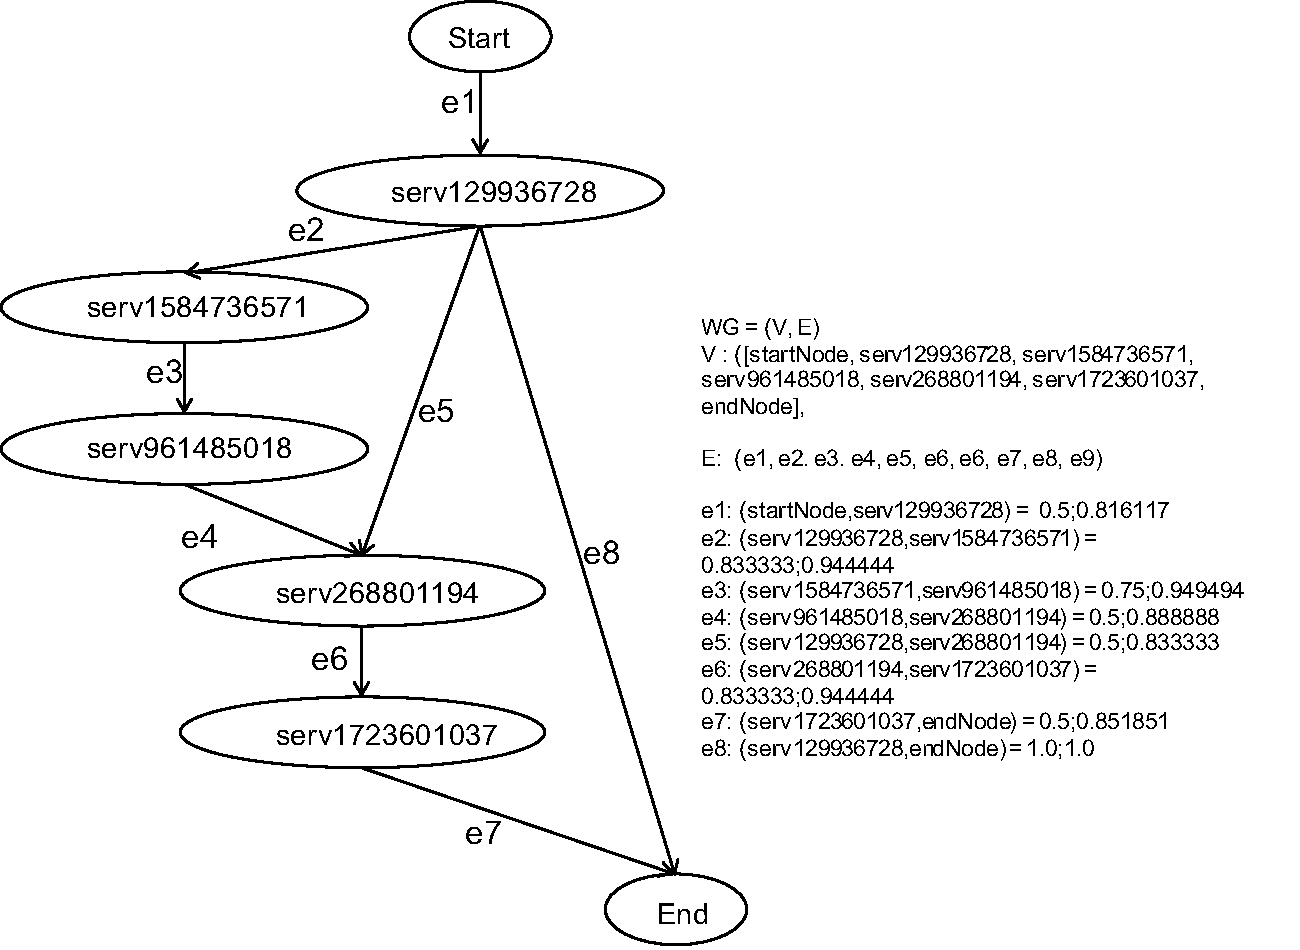
\includegraphics[scale=.29]{weigtedGraphExample.pdf}}
 \caption{Composition weighted graph solution}
 \label{wscs}
\end{figure}

\subsection{Fitness Calculation}
The fitness value of a service composition solution is a weighted sum of all the quality related components in Formula (\ref{equation6}), in which fitness value of 1 means the best comprehensive quality and 0 means the worst. For this purpose, $MT$, $S$, $A$, $R$, $T$, and $C$ must be normalised so that the fitness value falls within the range from 0 to 1. Therefore, the service composition problem in this paper is treated as a fitness maximisation problem.
\vspace{-0.2cm}
\begin{equation}
\label{equation6}
Fitness = w_1 \hat{MT} + w_2 \hat{S} + w_3 \hat{A} + w_4 \hat{R} + w_5(1 - \hat{T}) + w_6(1 - \hat{C})
\end{equation}
\noindent where $\sum_{i=1}^{6} w_i = 1$
\\
\vspace{-0.2cm}
\begin{equation}
\label{equation7}
\hat{Q_k} = 
\begin{cases}
	\frac{Q_k - Q_{k, min}}{Q_{k, max} - Q_{k, min}} & \text{ if }Q_{k, max} - Q_{k, min} \neq 0.\\
	1 & \mathrm{ otherwise}.
\end{cases}
\end{equation}
\noindent where $k$ $=$ $1$, $2$, $3$, and $4$, where $Q_1$ as $MT$, $Q_2$ as $S$, $Q_3$ as $A$, and $Q_4$ as $R$.
\begin{equation}
\label{equation8}
\hat{Q_j} = 
\begin{cases}
	\frac{Q_{j,max} - Q_j}{Q_{j, max} - Q_{j, min}} & \text{ if }Q_{j, max} - Q_{j, min} \neq 0.\\
	1 & \mathrm{ otherwise}.
\end{cases}
\end{equation}
\noindent where $j$ $=$ $1$, and $2$, where $Q_1$ as $T$ and $Q_2$ as $C$.


\subsection{QoS-aware Semantic Web Service Composition Algorithm} \label{pso_algorithm}
\begin{algorithm}[!htb]
 \setlength\hsize{0.9\linewidth}
 \SetKwInOut{Input}{Input}\SetKwInOut{Output}{Output}
 \let\oldnl\nl% Store \nl in \oldnl
\newcommand{\nonl}{\renewcommand{\nl}{\let\nl\oldnl}}
 \LinesNumbered
 	\textbf{1.} Map each relevant service to an index in the particle's position vector.\\
	\textbf{2.} Randomly initialise each particle in the swarm.\\
	\nonl \While {max. iterations not met}{
		\ForAll{particles in the swarm}{
		    \textbf{3.} Create queue of services using the particle's position vector.\\
			\textcolor{blue}{\textbf{4.} Build a weighted graph using the queue.}\\
			\textcolor{blue}{\textbf{5.} Calculate the fitness of the weighted graph.}\\
			\eIf{fitness value better than pBest}{
				\textbf{6a.} Assign current fitness as new pBest.\\
			}{
				\textbf{6b.} Keep previous pBest.\\
			}		
		}
		\textbf{7.} Assign best particle's \emph{pBest} value to \emph{gBest}, if better than gBest.\\
		\textbf{8.} Calculate the velocity of each particle according to the equation:\\
		\Indp $v_{id} = v_{id} + c_1 * rand() * (p_{id} - x_{id}) + c_2 * rand() * (p_{gd} - x_{id})$\\
		\Indm \textbf{9.} Update the position of each particle according to the equation:\\
		\Indp $x_{id} = x_{id} + v_{id}$\\
	}
	
 \caption{Steps of the PSO-based Web service composition technique.}
\label{novelSteps}

\end{algorithm}
\begin{algorithm}[!htb]
 \setlength\hsize{0.9\linewidth}
 \SetKwInOut{Input}{Input}\SetKwInOut{Output}{Output}
 \let\oldnl\nl% Store \nl in \oldnl
\newcommand{\nonl}{\renewcommand{\nl}{\let\nl\oldnl}}
 \Input{$I$, $O$, $queue$}
 \Output{composition weighted graph $WG$}
 \textbf{1.} Create $start$ vertex with outputs $O$ and $end$ vertex with inputs $I$.\\
 \textbf{2.} Create graph $WG$ containing the $start$ vertex.\\
 \textbf{3.} Create available outputs set containing $start$ outputs.\\
 \While{available outputs do not satisfy $end$ inputs}{
 \textbf{4.} Get next candidate from queue.\\
 \If{candidate inputs are satisfied by available outputs}{
 \textcolor{blue}{\textbf{5.} Create edge assigned with weight.\\}
 \textcolor{blue}{\textbf{6.} Connect vertex to graph with the edge.\\}
 \textbf{7.} Remove it from queue and go back to the queue's beginning.\\
 }}
 \textbf{8.} Connect end vertex.\\
 \textbf{9.} Remove dangling vertices from graph $WG$.\\
 \textcolor{blue}{\textbf{10.} Remove dangling edges from graph $WG$.\\}
 \KwRet $WG$.\\
 \caption{Create a composition weighted graph from a queue}	
\label{graph_building}
\end{algorithm}

The overall algorithm investigated here is made up of a PSO-based web service composition algorithm \ref{novelSteps} and a decoding algorithm \ref{graph_building}, to generate a composition weighted graph, where code lines in blue are different from the algorithm in \cite{da2016particle}. In algorithm \ref{novelSteps}, the idea is to translate the particle location produced by PSO into a service queue as an indirect representation of weighted graph, such that finding the best fitness of the weighted graph is to discover the optimised location of the particle in the search space. In PSO, the dimension of each particle equals to the number of relevant web services. The index of each services is mapped to a separate location component in a particle. Services in a queue follow the ascending order, from which we decode a weighted graph using Algorithm \ref{graph_building}. We select and connect  service vertex to the start vertex from the service queue if the web service can satisfy the output of start vertex. Meanwhile, an Output Set is initialised and kept being updated using outputs from the newly added service vertex in the weighted graph, later on, more services vertices are connected with edges if services' inputs could be satisfied by any output in the Output Set. Finally, the end vertex is connected to the graph if the updated Output Set contains all end inputs. In addition, dangling service vertex and edges will be removed. 
\section{Experiment Design}\label{experiment_design}
In this section, a quantitative evaluation approach is adopted in our experiment design. The objectives of the evaluation are to $(1)$ measure the effectiveness of the comprehensive quality model in automated semantic web service composition approach; $(2)$ explore the impacts of the semantic matchmaking that contributes to overall composition quality; and $(3)$ compare solutions generated by QoS-ware approach with our method.

We utilise benchmark dataset web service challenge 2009 (WSC09) \cite{kona2009wsc} to perform the evaluation. WSC09 provides problems with five tasks corresponding to variable number of services, and ontologies. Therefore, it is a challenge dataset for measuring the scalability of our quality evaluation model. Table \ref{wsc09datasetTable} presents the features of the WSC’09 dataset. The number of concepts, individuals in the ontology and services in each data set is shown in the second, third, fourth column respectively. Also, we extend all the datasets with QoS attributes from service providers to enable our evaluation. 

\begin{table}[]
\centering
\caption{Features of the WSC09 datasets}
\label{wsc09datasetTable}
\begin{tabular}{l|l|l|l}
\hline
\multicolumn{1}{c|}{Dataset} & No.Concept & No.Individual & No.Service \\ \hline
WSC09 01                     & 1578       &3102           &572      \\ \hline
WSC09 02                     & 12388      &24815          &4129      \\ \hline
WSC09 03                     & 18573      &37316          &8138      \\ \hline
WSC09 04                     & 18673      &37324          &8301      \\ \hline
WSC09 05                     & 31044      &62132          &15211    \\ \hline
\end{tabular}
\end{table}

We run the experiment on computing grid comprising of 170 NetBSD (Unix operating system) workstations operated by the Sun Grid Engine. The parameters were chosen based on general settings from \cite{shi2001particle} for our PSO-based approach, In particular, PSO population size is 30 with 100 generations. We run 30 times independently for each dataset. We configure weight of fitness function to properly balance functional side and nonfunctional side. Therefore, $w_{1}$ and $w_{2}$ equal to 0.1 and 0.4,  and $w_{3}$, $w_{4}$, $w_{5}$, $w_{6}$ are all set to 0.125 accordingly. However, the settings of these weight values does not impact the method. In general, weight settings are adjusted according to users' preferences.


\section{Results and Analysis}\label{results_analysis}
\subsection{Comparison Test with QoS Evaluation Model}\label{comparisonTest}
In this section, we analyse the composition solution generated by using our approach comparing with QoS-aware approach. In particularly, we show that our proposed approach can produce solutions that results in better matchmaking, which meets user's goal better.
 
First, we look at mean value of $Q_{mt}$, $Q_{s}$ and $Q_{QoS}$ at optimum at the 100th generation for two approaches, shown in Table \ref{decisionTable}. The QoS-aware approach record $Q_{mt}$, $Q_{s}$ and utilise fitness function $Fitness = w_1 \hat{A} + w_2 \hat{R} + w_3(1 - \hat{T}) + w_4(1 - \hat{C})$ when $\sum_{i=1}^{4} w_i = 1$ without considering $MT$ and $S$, in which $Q_(QoS)$ is normalised from 0 to 0.5 to make it comparable to $Q_{QoS}$ in our approach. We observe an interesting pattern from Table \ref{decisionTable} using statistic analysis: mean value of $Q_{mt}$ and $Q_{s}$ at optimum by our approach is consistently higher than those by QoS-aware approach with one exception in Task 2 while the combination of mean $Q_{mt}$ and $Q_{s}$ at optimum in Task 2 is still significantly higher in our approach under statistical anlysis. Meanwhile, $Q_{QoS}$ generated by QoS-aware approach can obtain a slightly higher value than that of our approach. In conclusion, we can perceive that our evaluation could find out better functional quality with a reasonable trade off in QoS.
\begin{table}[]
\footnotesize
\centering
\caption{Mean Quality for comprehensive quality-aware methods and QoS-aware approach}
\label{decisionTable}
\begin{tabular}{l|l|l|l}
\hline
\multicolumn{2}{c|}{WSC09}              & \shortstack{QoS-aware \\ Evaluation} & \shortstack{Comprehensive \\ Quality Evaluation} \\ \hline
\multirow{3}{*}{Task1}  &$Q_{mt}$   &0.189787 $\pm$ 0.039278686  &0.220594 $\pm$ 0.009318 $\uparrow$ \\ \cline{2-4} 
                        &$Q_{s}$    &0.884962 $\pm$ 0.014140   &0.893713 $\pm$ 0.007769  $\uparrow$ \\ \cline{2-4}
                        &$Q_{QoS}$  &0.278730 $\pm$ 0.007786     &0.279548 $\pm$ 0.007627                          \\ \hline
\multirow{3}{*}{Task2}  &$Q_{mt}$   &0.001795 $\pm$ 0.000719 $\uparrow$    &0.001135 $\pm$ 0.000633  \\ \cline{2-4} 
                        &$Q_{s}$    &0.906971 $\pm$ 0.005855     &0.927965 $\pm$ 0.007306 $\uparrow$   \\ \cline{2-4}
                        &$Q_{QoS}$  &0.239979 $\pm$ 0.000578 $\uparrow$     &0.237845 $\pm$ 0.001439 \\ \hline
\multirow{3}{*}{Task3}  &$Q_{mt}$   &0.158526 $\pm$ 0.014028               &  0.245830 $\pm$ 0.007761 $\uparrow$   \\ \cline{2-4} 
                        &$Q_{s}$    &0.949109 $\pm$ 0.002331           &   0.972765 $\pm$ 0.002980 $\uparrow$           \\ \cline{2-4}
                        &$Q_{QoS}$  &0.247002 $\pm$ 0.000661 $\uparrow$             &  0.245631 $\pm$ 0.000431            \\ \hline
\multirow{3}{*}{Task4}  &$Q_{mt}$   &0.000000 $\pm$ 0.000000  &0.000001 $\pm$ 0.000002 $\uparrow$ \\ \cline{2-4} 
                        &$Q_{s}$    &0.880058 $\pm$ 0.006603    &0.930632 $\pm$ 0.009043 $\uparrow$ \\ \cline{2-4}
                        &$Q_{QoS}$  &0.242338 $\pm$ 0.000516 $\uparrow$    &0.236677 $\pm$ 0.002211  \\ \hline
\multirow{3}{*}{Task5}  &$Q_{mt}$   &  0.000042 $\pm$ 0.000030     &  0.000078 $\pm$ 0.000031 $\uparrow$           \\ \cline{2-4} 
                        &$Q_{s}$    &  0.915933 $\pm$ 0.012888      &  0.928189 $\pm$ 0.002486 $\uparrow$                 \\ \cline{2-4}
                        &$Q_{QoS}$  & 0.238189 $\pm$ 0.000240$\uparrow$      &  0.237232 $\pm$  0.000391  \\ \hline                                                   
\end{tabular}
\end{table}

Second, to compare the results generated from two evaluation approaches, we demonstrate an example solution that shows the differences in composite web services obtained through two different methods. Fig. \ref{comparisontest} $(1)$ and $(2)$ show two composition weighted graphs as the solutions to Task 3 with $(1)$ QoS-aware approach and $(2)$ Comprehensive quality-aware method respectively. Two approaches generate exactly the same service workflow structure where those service vertices and edges denoted in red are different. We make a comparison of the quality among these different edges ($e_1$ to $e4$) associated service vertices in terms of quality of semantic matchmaking and QoS attributes in Fig. \ref{comparisontest} $(3)$. We also look at $\Delta Q$ which reveals the amount of variation on quality between two methods, where the positive values means the benefits gained under our approach while the negative values means the trade-off. To demonstrate the benefits of the positive value, we analyse the smallest positive $\Delta Q$ corresponding to $e_4$ and demonstrate how the output and required input are different under two approaches in Fig. \ref{comparisontest} $(4)$. $Ser1640238160$ and $Ser1947554374$ are selected service vertices with output concept-related parameters $Inst795998200$ and $Inst582785907$ corresponding to two concepts $Con103314376$ and $Con2037585750$ respectively, and $Inst658772240$ are the required parameter related to concept $Con2113572083$. There exist $Inst795998200$ $\in$ $Con103314376$ $\sqsubseteq_{2}$ $Inst658772240$ $\in$ $Con2113572083$ and $Inst582785907$ $\in$ $Con2037585750$ $\sqsubseteq_{3}$ $Inst658772240$ $\in$ $Con2113572083$. It is obvious that our approach selects the service providing $Inst795998200$ that are closer to the users' requirements suggesting that our method can produce better semantic matchmaking quality.

\begin{figure}[h]
\centering{
\fbox{
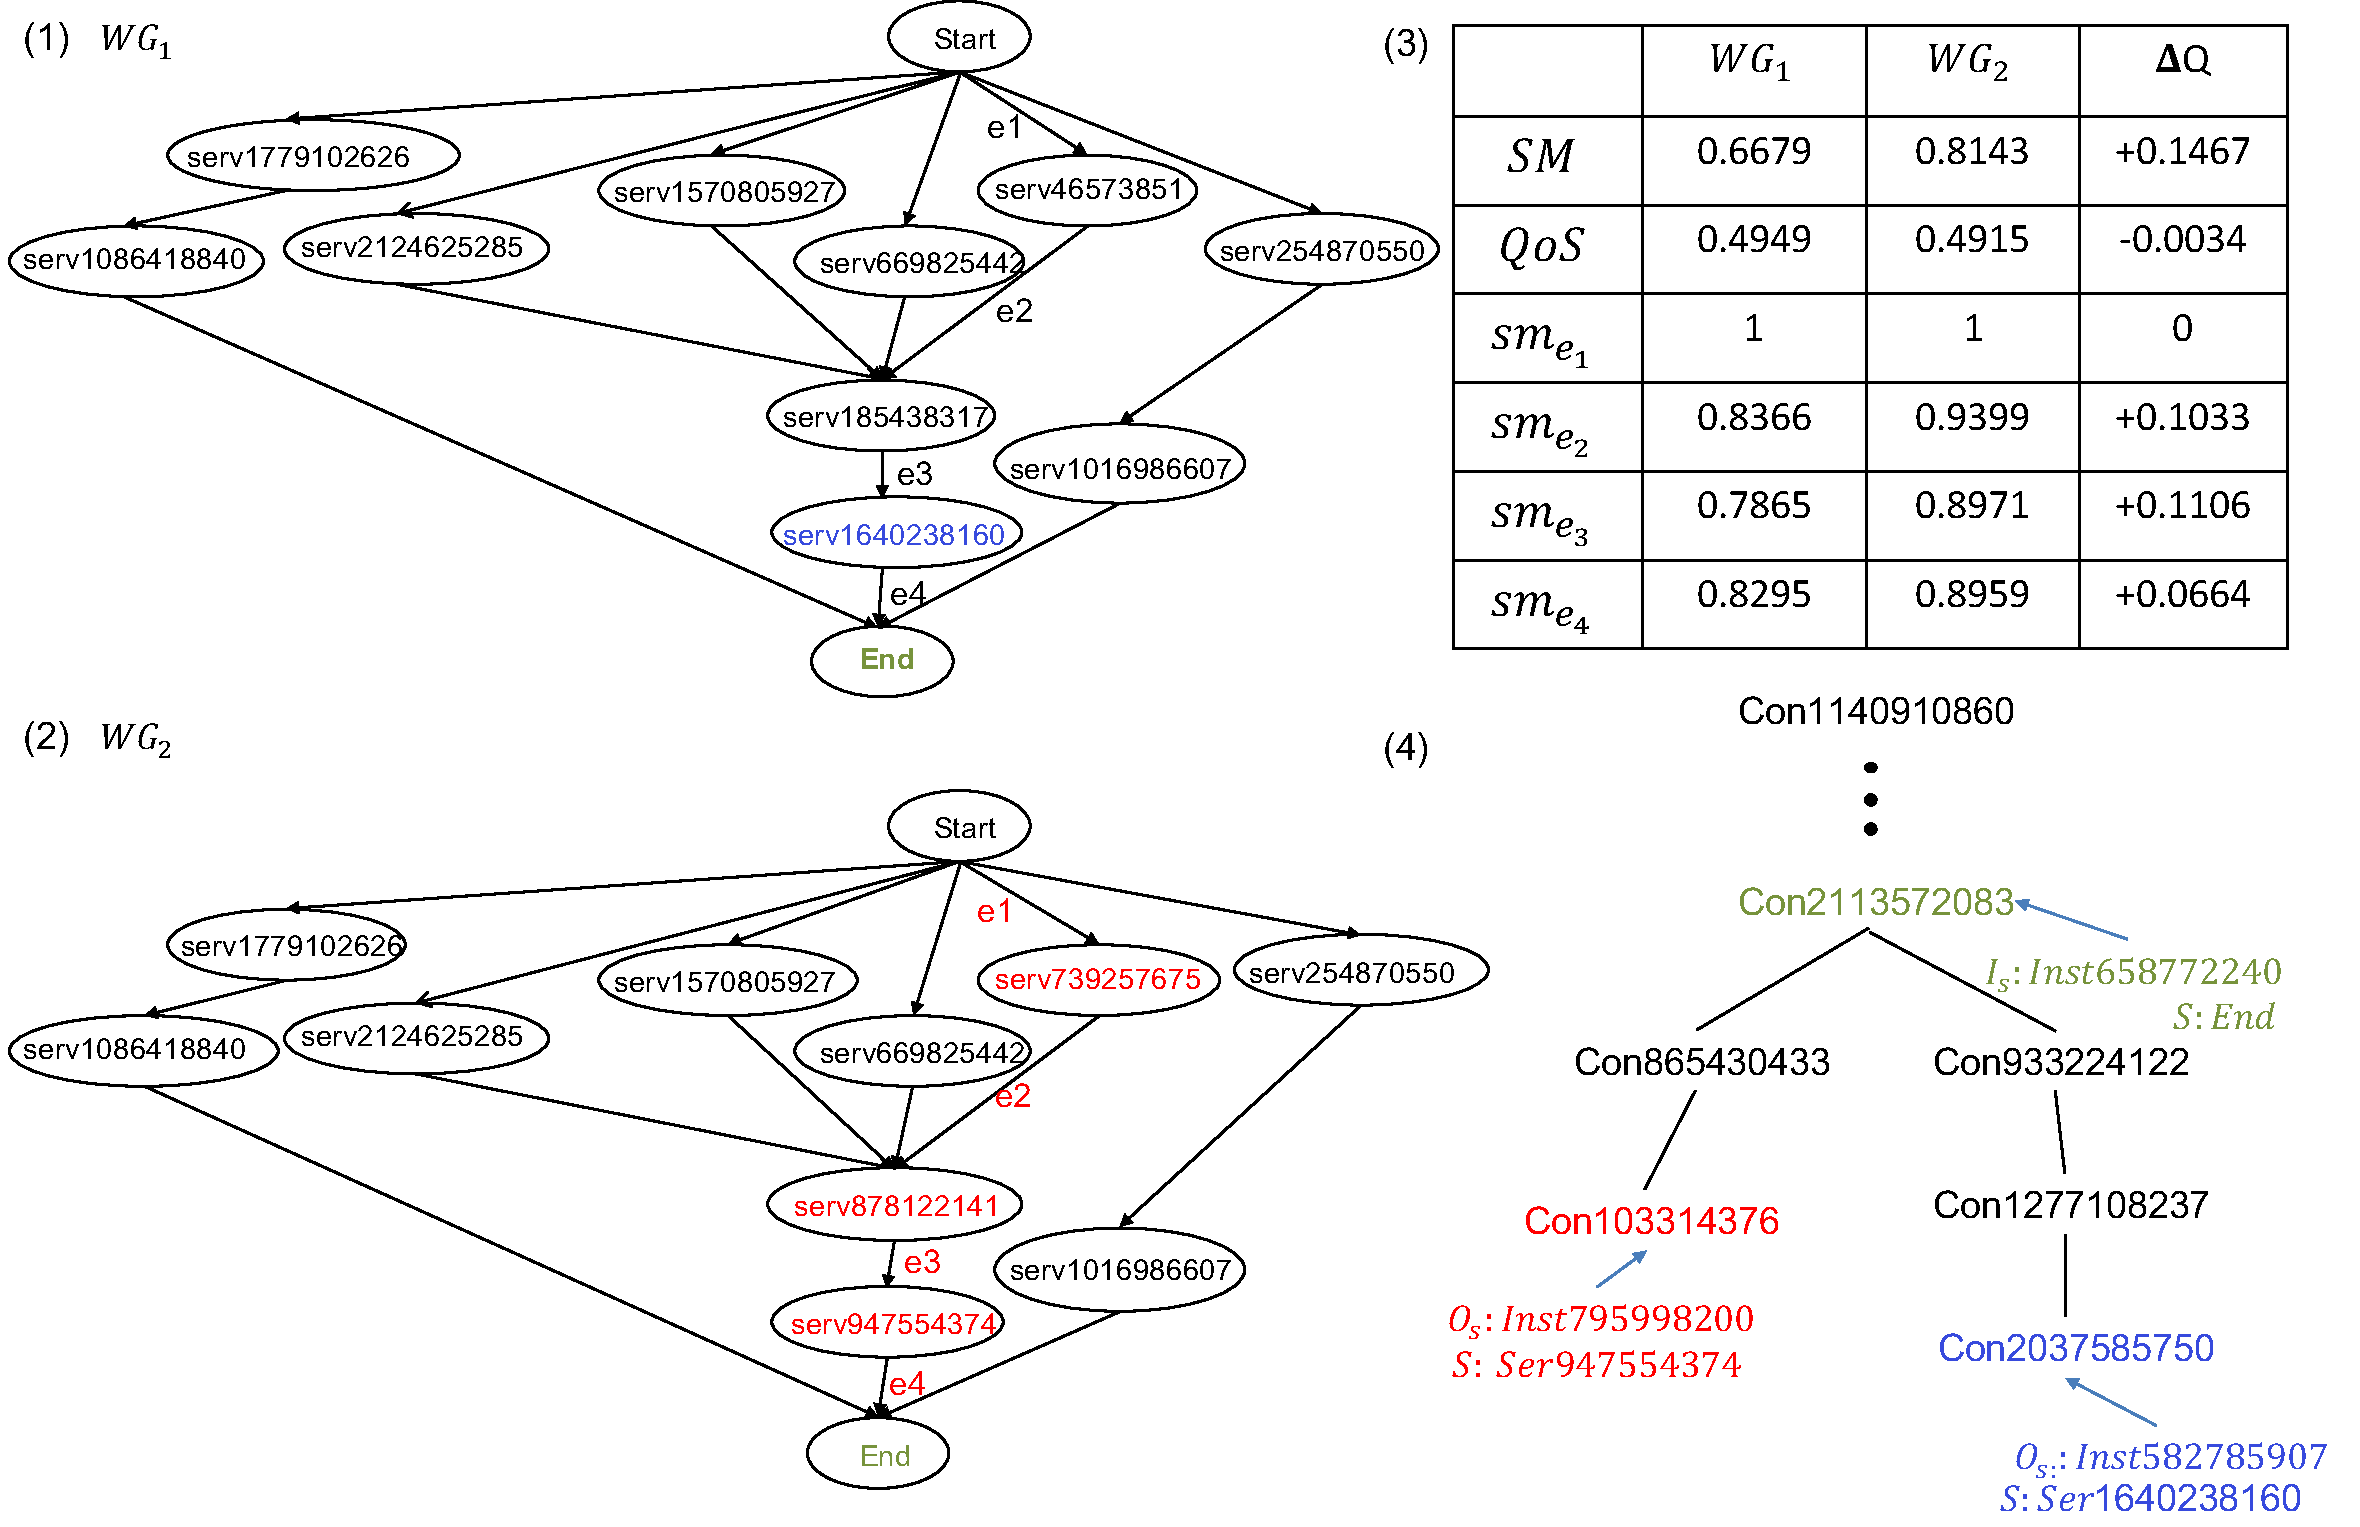
\includegraphics[scale=.22]{comparisontest.pdf}}}
 \caption{Example Comparison of solutions to Task 3 under different approaches.}
 \label{comparisontest}
\end{figure}

\subsection{Convergence Test}\label{convergenceTest}
To analyse the effectiveness of our approach, we study the convergence rate of the proposed method in this section to understand the convergence rate of five tasks in WSC09. We analysis the performances during the whole evolutionary process in Fig. \ref{exp_fitnessvalue}, in which experiment results on five tasks are arranged in four groups consisting of average fitness, average matchType quality, average similarity quality and average QoS for generation 0-99 with optimum.

\begin{figure}[h]
\centering{
\fbox{
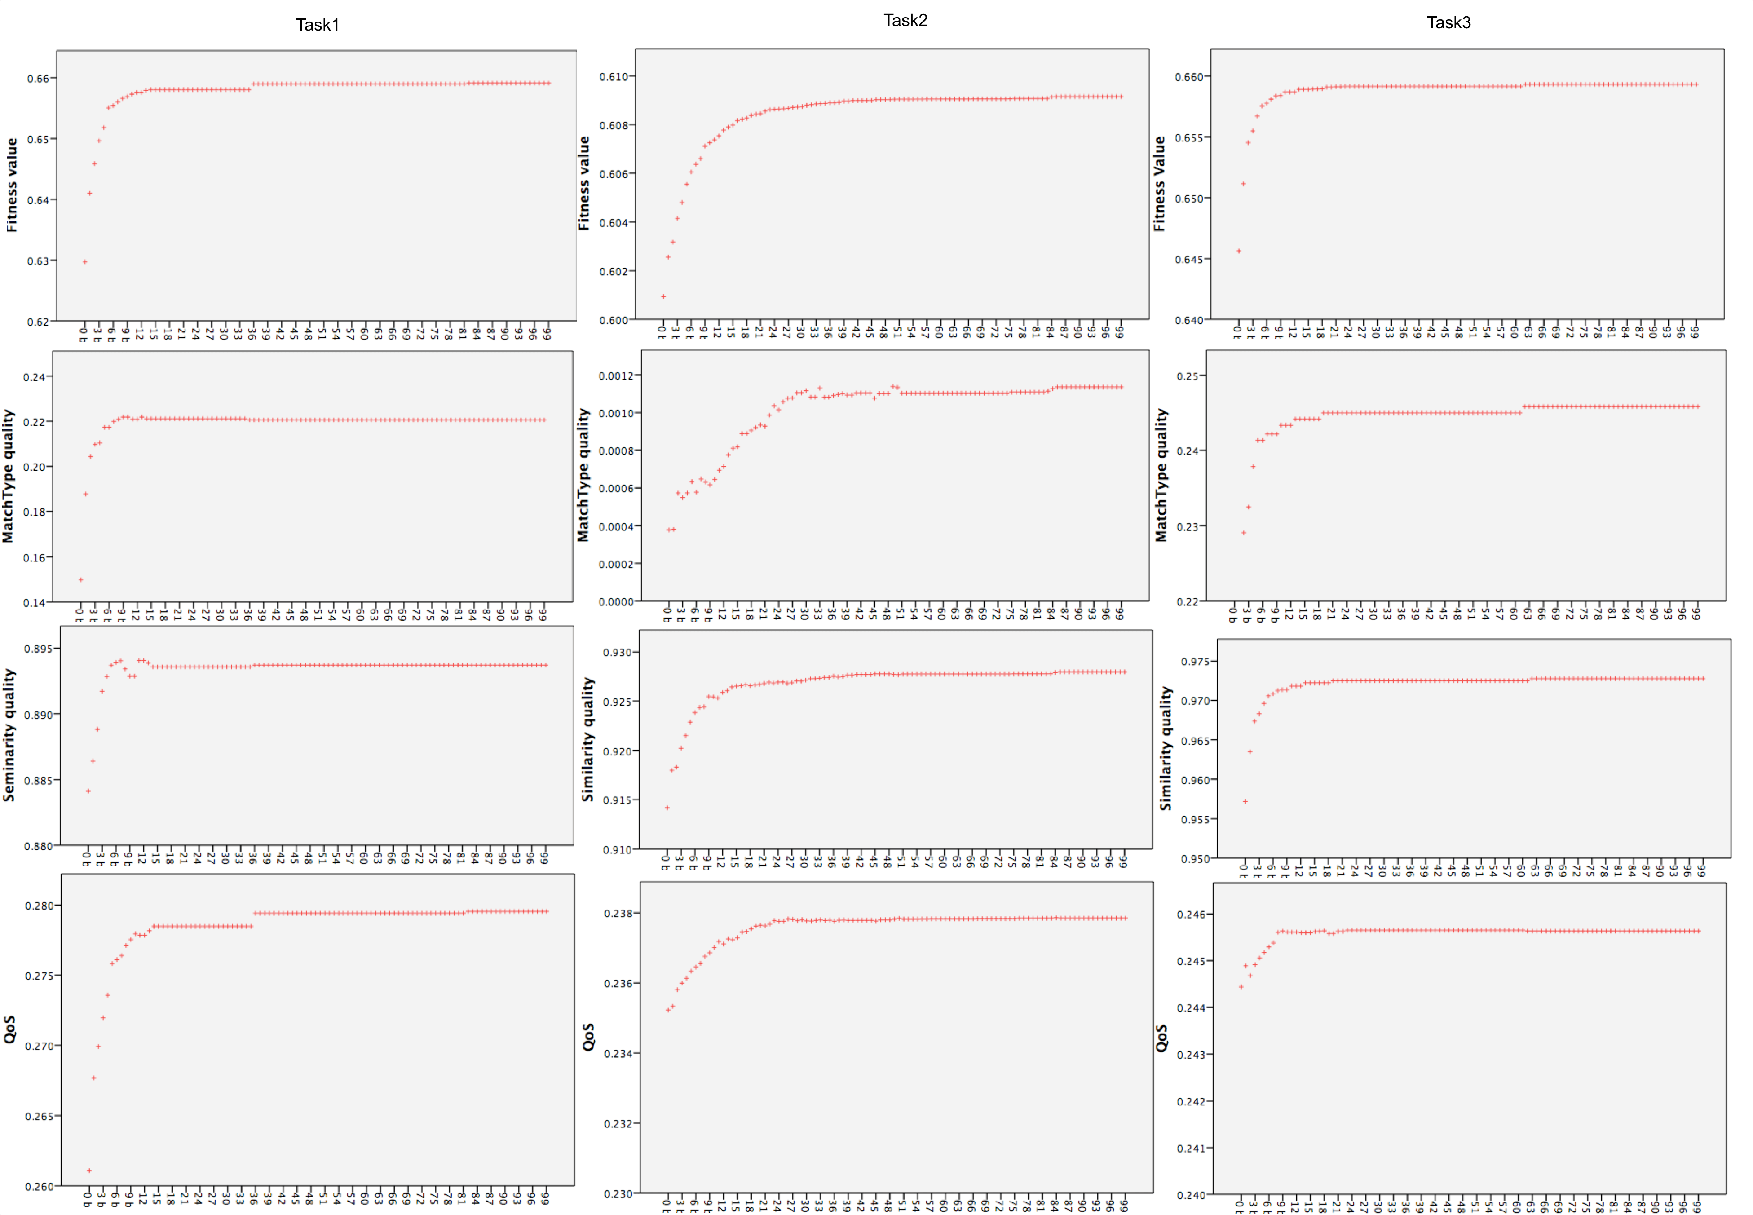
\includegraphics[scale=.095]{convergency.pdf}}}
 \caption{Average Fitness, Average MatchType Quality, Average Similarity quality and Average QoS per generation with comprehensive quality optimum}
 \label{exp_fitnessvalue}
\end{figure}
Firstly, the average fitness value with optimum is calculated by averaging the best fitness found in each generation over 30 independent runs. We can see that there is a significant increase in the fitness values towards optimum between generation 0 and generation 15-25, the remaining generation continues to produce a steady but moderate improvement in the fitness value and eventually reach a plateau with no further improvements can be observed. The same behaviour is observed over the rest tasks.

We also investigate the variation of quality of semantic matchmaking where average matchType quality with optimum and average similarity quality with optimum are studied from generation 0 to 99 in second and third column groups of Fig. \ref{exp_fitnessvalue}. In these subfigures, both the average matchType quality with optimum and average similarity quality with optimum refers to the mean values of the quality values associated to the best fitness value found in each generation over 30 independent runs. Similar to the fitness values, clear evidence of fast convergence can be observed with respect to theses quality values. This observation is also consistent for the improvement of mean QoS quality with optimum shown in the last column in Fig \ref{exp_fitnessvalue}. Additionally, we don't see too much trade-off from the QoS as the a consistently increase in semantic matchmaking quality is observed.


\subsection{Comparison Test with GP-based approach}\label{comparisonTestWithGP}
We compare a GP-based approach  \cite{ma2015hybrid} with our PSO method, where the individual is a tree structure transferred from a DAG employing unfolding techniques. We further mark all the tree nodes in the representation with its outgoing edges for semantic matchmaking quality, and those edges information are maintained correctly throughout the evolutionary process. At last, we evaluate both semantic matchmaking quality and QoS simultaneously using the discussed the comprehensive quality model to investigate the performances of both GP-based approaches and PSO-based approach. To make a fair comparison with our PSO approach that the same number of evaluations (3000 times) should be considered, we adjust the parameters settings for GP approach \cite{ma2015hybrid} to 30 individual for 100 generations.

The Table \ref{meanFitness} shows the mean fitness values accomplished by two methods and Table \ref{meanTime} shows the average execution time required by them. We employ statistical analysis to test the significant differences in mean fitness value and execution time.  The results show that the PSO-based approach performs better in four of five tasks. However, there is also a trade-off between optimised solution and execution time. We can see the PSO-based approach takes longer execution time, it due to that the every individual in each generation must be decoded from generated optimised queue, and this process is very time-consuming. However,  the initialisation first population in GP-based approach is costly in time as transformation process from a DAG, but following new individuals are generated through mutation and crossover, which are considered be much less time consumed comparing decoding process.

\begin{table}[]
\centering
\caption{Mean fitness results for comparing GP-based approach}
\label{meanFitness}
\begin{tabular}{l|l|l}
\hline
\multicolumn{1}{c|}{Dataset} & PSO-based approach & GP-based approach  \\ \hline
WSC09 01                     &0.559207 $\pm$ 0.012780 $\uparrow$      &0.518411 $\pm$ 0.018470               \\ \hline
WSC09 02                     &0.470083 $\pm$  0.001106   &0.471594 $\pm$  0.002436 $\uparrow$           \\ \hline
WSC09 03                     & 0.559207 $\pm$ 0.012780 $\pm$ $\uparrow$  &0.552947 $\pm$ 0.007094            \\ \hline
WSC09 04                     & 0.468942 $\pm$ 0.001670 $\pm$ $\uparrow$  &0.442934 $\pm$ 0.010154            \\ \hline
WSC09 05                     & 0.469424 $\pm$ 0.000800 $\pm$ $\uparrow$  &0.256425 $\pm$ 0.038916            \\ \hline
\end{tabular}
\end{table}


\begin{table}[]
\centering
\caption{Mean time results for comparing GP-based approach}
\label{meanTime}
\begin{tabular}{l|l|l}
\hline
\multicolumn{1}{c|}{Dataset} & PSO-based approach & GP-based approach  \\ \hline
WSC09 01                     &12907 $\pm$ 8105      &5168 $\pm$ 520 $\downarrow$                \\ \hline
WSC09 02                     &292346 $\pm$  96727    &27483 $\pm$  3083 $\downarrow$          \\ \hline
WSC09 03                     & 12908 $\pm$ 8105 $\downarrow$  &28053 $\pm$ 3202            \\ \hline
WSC09 04                     & 6553640 $\pm$ 1468204   &540418 $\pm$ 186540 $\downarrow$            \\ \hline
WSC09 05                     & 1208193 $\pm$ 266916   &180408 $\pm$ 435247 $\downarrow$           \\ \hline
\end{tabular}
\end{table}

\begin{figure}[h]
\centering
\fbox{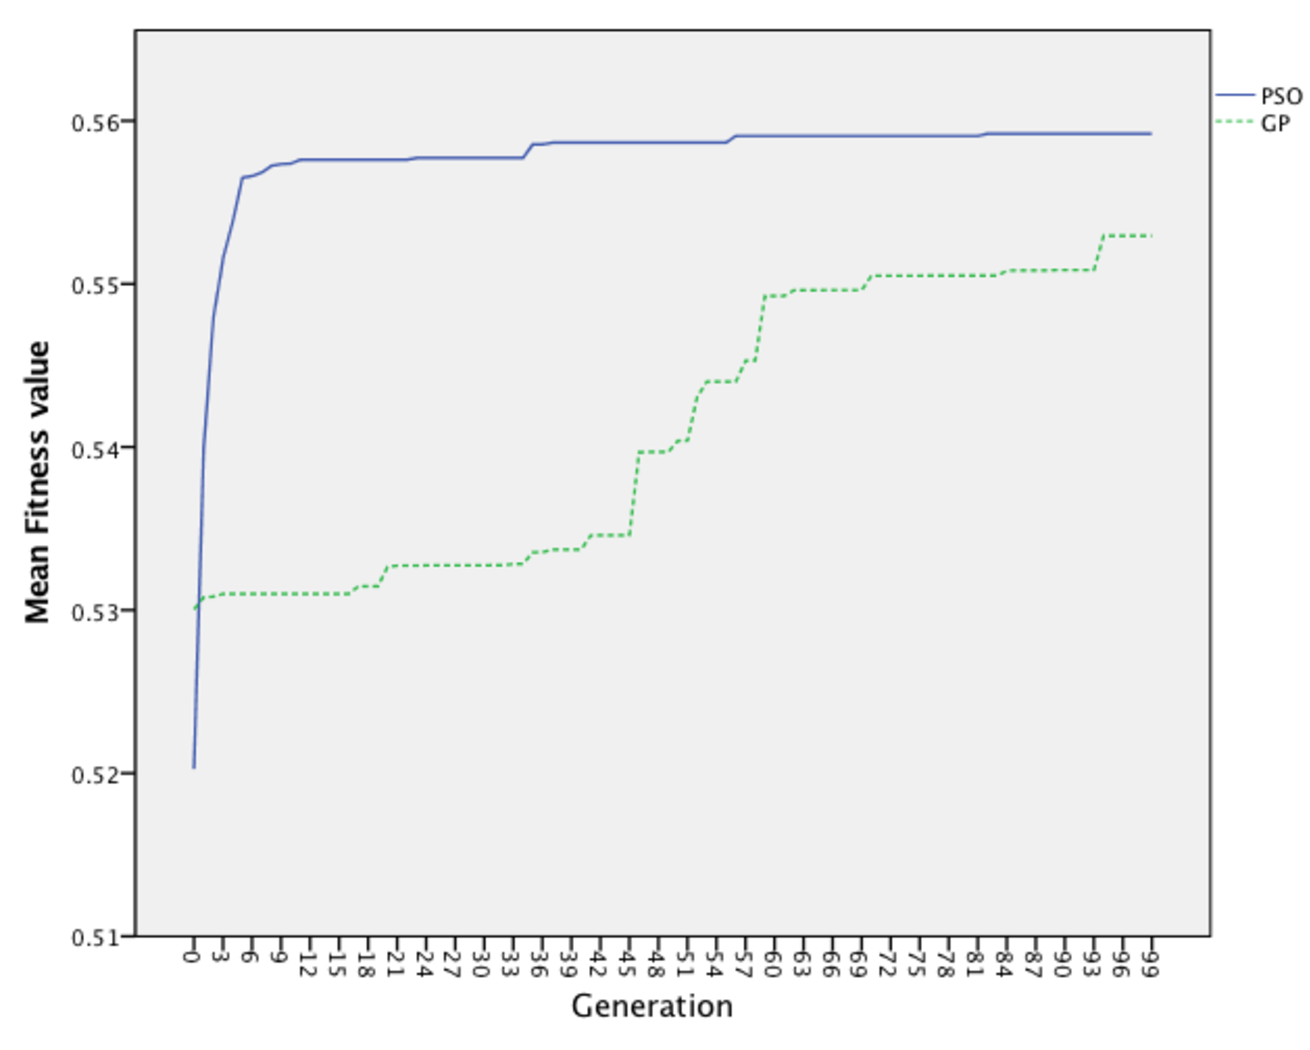
\includegraphics[scale=.25]{psovsgp.pdf}}
 \caption{An example of comparing convergency rate from PSO and GP approaches for task 3}
 \label{psovsgp}
\end{figure}

We also study the average fitness value with the optimum through the evolutionary process for both PSO-based and GP-based approach over 30 independent runs. Fig. \ref{psovsgp} is an example of convergence rate from Task 3, where the behaviour of PSO-based approach presents a very clear evidence of fast convergence and reaches a better-optimised solution, while the performance of GP is barely satisfactory, as this method improves its fitness value gradually.

\section{Conclusion}\label{conclusion}
This work introduced an evaluation model for QoS-aware automated semantic automated web service composition that combines quality of semantic matchmaking with QoS. The results shows that our comprehensive quality model is proved to obtain better functional quality with a reasonable trade-off in QoS. Future works could explore the comprehensive quality with multi-objectives to maximising the quality of matchmaking and to optimise QoS, and to improve efficiency in calculating semantic matchmaking quality.
\bibliographystyle{IEEEtran}
\bibliography{IEEEexample}

\end{document}